\icode{E-MD-MU-L3-261120-001}
（多选）
如图所示，质量均为 \(m\) 的 \(A\)、\(B\) 两物体叠放在竖直弹簧上并保持静止，现对 \(B\) 物体施加竖直向上的拉力使 \(B\) 物体以加速度 \(\frac{g}{2}\) 做匀加速直线运动，直到 \(B\) 与 \(A\) 刚分离。下列说法中正确的是\paren[]

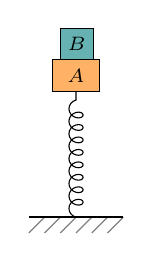
\begin{tikzpicture}[>=stealth,font=\scriptsize]
	\draw[decoration={aspect=.8,segment length=4.5,amplitude=.9mm,coil},decorate] (0,0)--(0,1.6);
	\draw[fill=orange!60] (-.3,1.6) rectangle(.3,2)node[midway]{\(A\)};
	\draw[fill=teal!60] (-.2,2) rectangle(.22,2.4)node[midway]{\(B\)};
	\foreach \x in {-.6,-.4,...,.6}
		\draw[gray] (\x,-.2)--++(.2,.2);
	\draw[thick] (-.6,0)--(.6,0);
\end{tikzpicture}
\begin{choices}
	\item 刚分离时，\(A\) 的加速度为\(\frac{g}{2}\)		
	\item 刚分离时，\(A\) 的加速度为 0
	\item 刚分离时，弹簧处于压缩状态
	\item 刚分离时，弹簧处于自然长
\end{choices}
\begin{answer}
    AC\qquad 提示：
\end{answer}